\documentclass{article}
\usepackage[utf8]{inputenc}
\usepackage[ngerman]{babel}

% Convenience improvements
\usepackage{csquotes}
\usepackage{enumitem}
\usepackage{amsmath}
\usepackage{amssymb}
\usepackage{mathtools}
\usepackage{tabularx}
\usepackage{multicol}

% Proper tables and centering for overfull ones
\usepackage{booktabs}
\usepackage{adjustbox}

% Change page/text dimensions, the package defaults work fine
\usepackage{geometry}

\usepackage{parskip}

% Drawings
\usepackage{tikz}
\usetikzlibrary{automata, arrows.meta, positioning}
\usepackage{pgfplots}
\pgfplotsset{compat=1.18}

% Adjust header and footer
\usepackage{fancyhdr}
\pagestyle{fancy}
\fancyhead[L]{Formal Models --- \textbf{Assignment 1}}
\fancyhead[R]{Laurenz Weixlbaumer (11804751)}
\fancyfoot[C]{}
\fancyfoot[R]{\thepage}
% Stop fancyhdr complaints
\setlength{\headheight}{12.5pt}

% Adjust tikz automata styling
\tikzset{
    ->,
    initial text=
}

\newcommand{\Deltaop}{\, \Delta\, }
\newcommand{\xor}{\, \oplus\, }
\newcommand{\id}{\text{id}}

\begin{document}

\paragraph{Exercise 1}

\begin{align*}
    S &= \{ s_0, s_1, s_2, s_3, s_4, s_5, s_6 \} \\
    I &= \{ s_0 \} \\
    \Sigma &= \{ a, b \} \\
    T &= \begin{aligned}\{ &(s_0, a, s_1), (s_0, b, s_2), (s_1, b, s_2), (s_1, a, s_3), \\&(s_2, a, s_1), (s_2, b, s_4), (s_3, a, s_5), (s_3, b, s_2), (s_4, a, s_1), \\&(s_4, b, s6), (s_5, a, s_5), (s_5, b, s_5), (s_6, b, s_6), (s_6, a, s_6) \}
    \end{aligned} \\
    F &= \{ s_0, s_1, s_2, s_3, s_4 \}
\end{align*}

\begin{center}
    \begin{tikzpicture}
        \node (s0) [state, accepting, initial] {$s_0$};
        \node (s1) [state, accepting, above right = of s0] {$s_1$};
        \node (s2) [state, accepting, below right = of s0] {$s_2$};
        \node (s3) [state, accepting, right = of s1] {$s_3$};
        \node (s4) [state, accepting, right = of s2] {$s_4$};
        \node (s5) [state, right = of s3] {$s_5$};
        \node (s6) [state, right = of s4] {$s_6$};

        \draw
            (s0) edge[above] node{a} (s1)
            (s0) edge[below] node{b} (s2)
            (s1) edge[bend right=10, left] node{b} (s2)
            (s1) edge[above] node{a} (s3)
            (s2) edge[bend right=10, right] node{a} (s1)
            (s2) edge[below] node{b} (s4)
            (s3) edge[above] node{a} (s5)
            (s3) edge[right] node{b} (s2)
            (s4) edge[below] node{b} (s6)
            (s4) edge[left] node{a} (s1)
            (s5) edge[loop below] node{a, b} (s5)
            (s6) edge[loop above] node{a, b} (s6)
            ;
    \end{tikzpicture}
\end{center}

The automaton has one initial state and every state has exactly one successor state for every possible input. It is thus complete (at least one initial state and at least one successor) and deterministic (at most one initial state, at most one successor).

\paragraph{Exercise 2}

\begin{center}
    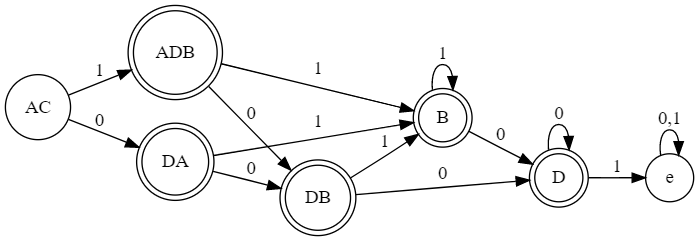
\includegraphics[width=.8\textwidth]{2_power.png}
\end{center}

\paragraph{Exercise 3}

The automaton $A$

\begin{center}
    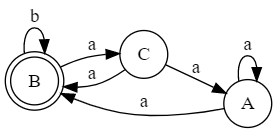
\includegraphics[width=.35\textwidth]{3_initial.png}
\end{center}

is neither deterministic nor complete. To determine the complement language, we use the power automaton

\begin{center}
    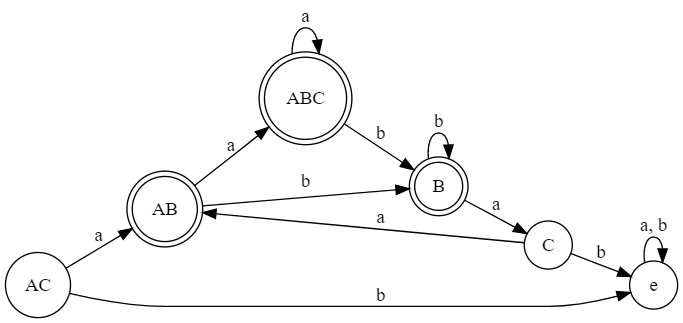
\includegraphics[width=.75\textwidth]{3_power.png}
\end{center}

with complement automaton.

\begin{center}
    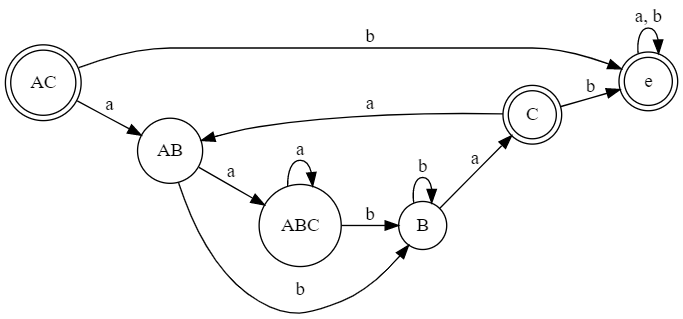
\includegraphics[width=.75\textwidth]{3_complement.png}
\end{center}

This automaton describes the complement language $\overline{L(A)}$.
\begin{align*}
    L(A) &= a(aa(a*)(b*))* \\
    K(A) = \overline{L(A)} &= \{ w \in \{a,b\}* : w \not\in L(A) \}
\end{align*}

\paragraph{Exercise 4}

\begin{center}
    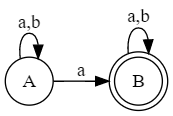
\includegraphics[width=.2\textwidth]{4_example.png}
\end{center}

The given automaton $A_3$ is neither complete nor deterministic. Because it has no initial state, we have $L(A_3) = L(C(A_3)) = \emptyset$ but $\overline{L(A_3)} = \{a,b\}^*$.

It can be made complete (but not deterministic) by adding an initial state. In this case $L(A_2) = \{a,b\}^* = L(C(A_2))$ but $\overline{L(A_2)} = \emptyset$. 

It can be made deterministic (but not complete) by removing the state B and the transition to it. In this case the argument for $A_3$ still holds.

\end{document}
